% Grid shares diagram (t = 2, n = 3)
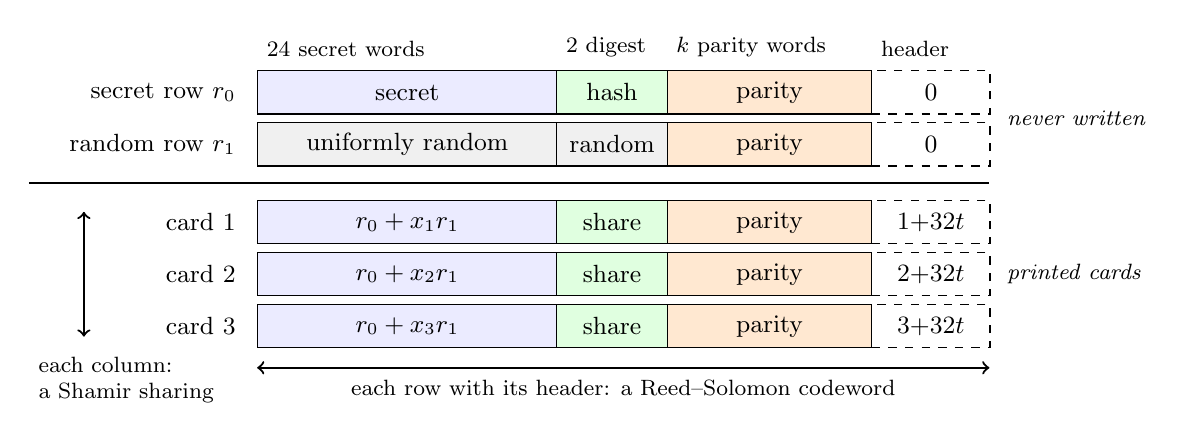
\begin{tikzpicture}[x=1cm,y=0.66cm,font=\small,
  cell/.style={draw,minimum height=0.55cm,inner sep=1pt,anchor=west},
  data/.style={cell,minimum width=3.8cm,fill=blue!8},
  dig/.style={cell,minimum width=1.4cm,fill=green!12},
  par/.style={cell,minimum width=2.6cm,fill=orange!18},
  hdr/.style={cell,minimum width=1.5cm,dashed}]
\node[anchor=south west,font=\footnotesize] at (0,0.5) {24 secret words};
\node[anchor=south west,font=\footnotesize] at (3.8,0.5) {2 digest};
\node[anchor=south west,font=\footnotesize] at (5.2,0.5) {$k$ parity words};
\node[anchor=south west,font=\footnotesize] at (7.8,0.5) {header};
\node[anchor=east] at (-0.15,0) {secret row $r_0$};
\node[data] at (0,0) {secret};
\node[dig] at (3.8,0) {hash};
\node[par] at (5.2,0) {parity};
\node[hdr] at (7.8,0) {0};
\node[anchor=east] at (-0.15,-1) {random row $r_1$};
\node[data,fill=gray!12] at (0,-1) {uniformly random};
\node[dig,fill=gray!12] at (3.8,-1) {random};
\node[par] at (5.2,-1) {parity};
\node[hdr] at (7.8,-1) {0};
\draw[thick] (-2.9,-1.75) -- (9.3,-1.75);
\node[anchor=west,font=\footnotesize\itshape] at (9.4,-0.5) {never written};
\node[anchor=west,font=\footnotesize\itshape] at (9.4,-3.5) {printed cards};
\foreach \i/\y in {1/-2.5,2/-3.5,3/-4.5}{
  \node[anchor=east] at (-0.15,\y) {card \i};
  \node[data] at (0,\y) {$r_0 + x_{\i} r_1$};
  \node[dig] at (3.8,\y) {share};
  \node[par] at (5.2,\y) {parity};
  \node[hdr] at (7.8,\y) {$\i{+}32t$};
}
\draw[<->,thick] (-2.2,-2.3) -- (-2.2,-4.7);
\node[anchor=north west,font=\footnotesize,align=left] at (-2.9,-4.9) {each column:\\ a Shamir sharing};
\draw[<->,thick] (0,-5.3) -- (9.3,-5.3);
\node[anchor=north,font=\footnotesize] at (4.65,-5.35) {each row with its header: a Reed--Solomon codeword};
\end{tikzpicture}
